\section{Methods}

Full atom simulations of DNA molecules exist but are computationally very heavy -- some methods even simulate the individual atoms of the solvent. These models yield of course a very high degree of detail, but the low computational efficiency forces these models to be useful only in describing small DNA oligomers (20-30 bp). LAMMPS \cite{plimpton2007lammps} is perhaps the most widespread of these tools, but other examples are the force-field based atomistic models like CHARMM \cite{brooks2009charmm} and AMBER \cite{cheatham1999modified}.

In 2007, the group of De Pablo \cite{knotts2007coarse} applied the technique of coarse graining to a molecular simulation of DNA: instead of simulating all atoms, a DNA monomer is represented by three sites or `beads': the sugar, the phosphate and the base. For simulations where one is mainly interested in the timescale behaviour or global dynamics of the DNA molecule this 3SPN (three-sites-per-nucleotide) model is a very good approximation: it is computationally cheap (and easy to optimize) while describing the DNA helical structure quite good. 

We implemented the 3SPN model with a few changes of our own: we adapted the model to implement space partitioning, we slightly modified the way base pairing forces were calculated and we custom-fitted some constants to better describe the zipping and unzipping dynamics of ssDNA hairpins.

The codebase was not available publicly, so everything had to be created from scratch in C with an OpenGL rendering engine attached --- we decided to make it open source and available at GitHub: \href{https://github.com/RoaldFre/DNA}{github.com/RoaldFre/DNA}. The interested reader can find the full package containing everything needed to reproduce the material presented in this paper at that location.



\subsection{DNA structure \label{secStructure}}

In this paper, we follow the approach of Knotts, De Pablo \etal \cite{knotts2007coarse} to model the structure of B-DNA. In Figure \ref{dna_forms}, the main three structural forms of DNA are illustrated.

\begin{figure}[htbp]
\begin{center}
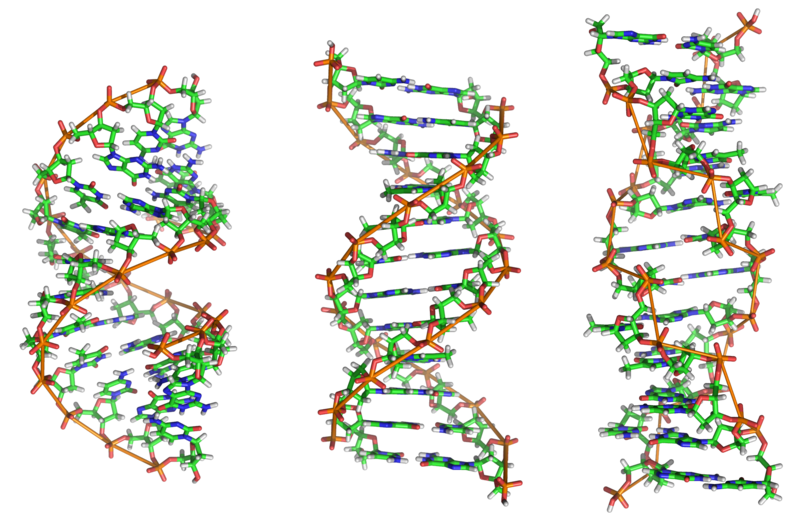
\includegraphics[width=14cm]{images/dna_forms.png}
\caption{Structural forms of DNA: A-DNA (left), B-DNA (center) and Z-DNA (right). Figure from \href{http://www.molecularstation.com}{molecularstation.com}.}
\label{dna_forms}
\end{center}
\end{figure}


The algorithm to build up a single strand is to follow the screw symmetry of B-DNA by placing consecutive monomers on the $z$-axis of space (separated by an axial rise of $3.38$\,\Angstrom), and rotating each consecutive monomer by an angle of $36$ degrees. In practice, this means that if a monomer is placed at location $(r, \phi, z)$, the consecutive monomer on the same strand is placed at $(r, \phi + 36\degree, z + 3.38\,\text{\Angstrom})$. To build up the complementary strand (yielding the characteristic double stranded helical structure of DNA), an atom at $(x, y, z)$ on the first strands has its complementary atom on the other strand at $(x, -y, -z)$ with the $x$-axis taken orthogonal to the helical axis and always along the line connecting the complementary bases of the complementary monomers (i.e. the $x$-axis also rotates $36\degree$ along the $z$-axis for consecutive base pairs along the double strand).

Knotts \etal \cite{knotts2007coarse} used the DNA molecular data of ref. \cite{crcBiochem1976}, and averaged positions for each of the three sites per nucleus yielding the data in table \ref{dnaStructureData}. Schematically, this structure yields the major and minor grooves as illustrated in Figure \ref{schematic_knotts}. The phosphate and sugar sites on the backbone of the molecule are placed at the centers of mass of the molecules; bases Ab and Gb are placed at the N1 position of the B-DNA isoform; bases Tb and Cb at the N3 position. 
\todo{because this is where the hydrogen bonds happen????}

\begin{table}[htdp]
\caption{Structural data for B-DNA helices, calculated by Knotts \etal \cite{knotts2007coarse}.}
\begin{center} \footnotesize
\begin{tabular}{|l|rrrrc|c|}
\hline
 &\ \  $x$ (\Angstrom)\ \ &\ \  $y$ (\Angstrom)\ \  &\ \  $z$ (\Angstrom)\ \  &\ \  $r$ (\Angstrom)\ \  &\ \  $\phi$ (degrees)\ \  & \ \ Mass (amu) \\
\hline
Phosphate (P) & -0.628 & 8.896 & 2.186 & 8.918 & 94.038 & 94.97 \\
Sugar (S) & 2.365 & 6.568 & 1.280 & 6.981 & 70.197 & 83.11 \\
Adenine base (Ab) & 0.575 & 0.516 & 0.051 & 0.773 & 41.905 & 134.1\\
Thymine base (Tb) & 0.159 & 2.344 & 0.191 & 2.349 & 86.119 & 125.1\\
Cytosine base (Cb) & 0.199 & 2.287 & 0.187 & 2.296 & 85.027 & 110.1\\
Guanine base (Gb) & 0.628 & 0.540 & 0.053 & 0.828 & 40.691 & 150.1\\
\hline
\end{tabular}
\end{center}
\label{dnaStructureData}
\end{table}%


At the beginning of the simulations, the world gets filled with a centered DNA helix of a given base sequence using the above algorithm. If requested, the complementary strand gets build and positioned correctly as well.

In Figure \ref{methods_dnaStructure} two screenshots of our implemented model are given, showing a side view of the double helix structure and a top view of the internal structure of the bond and dihedral angles.


\begin{figure}[h]
\begin{center}
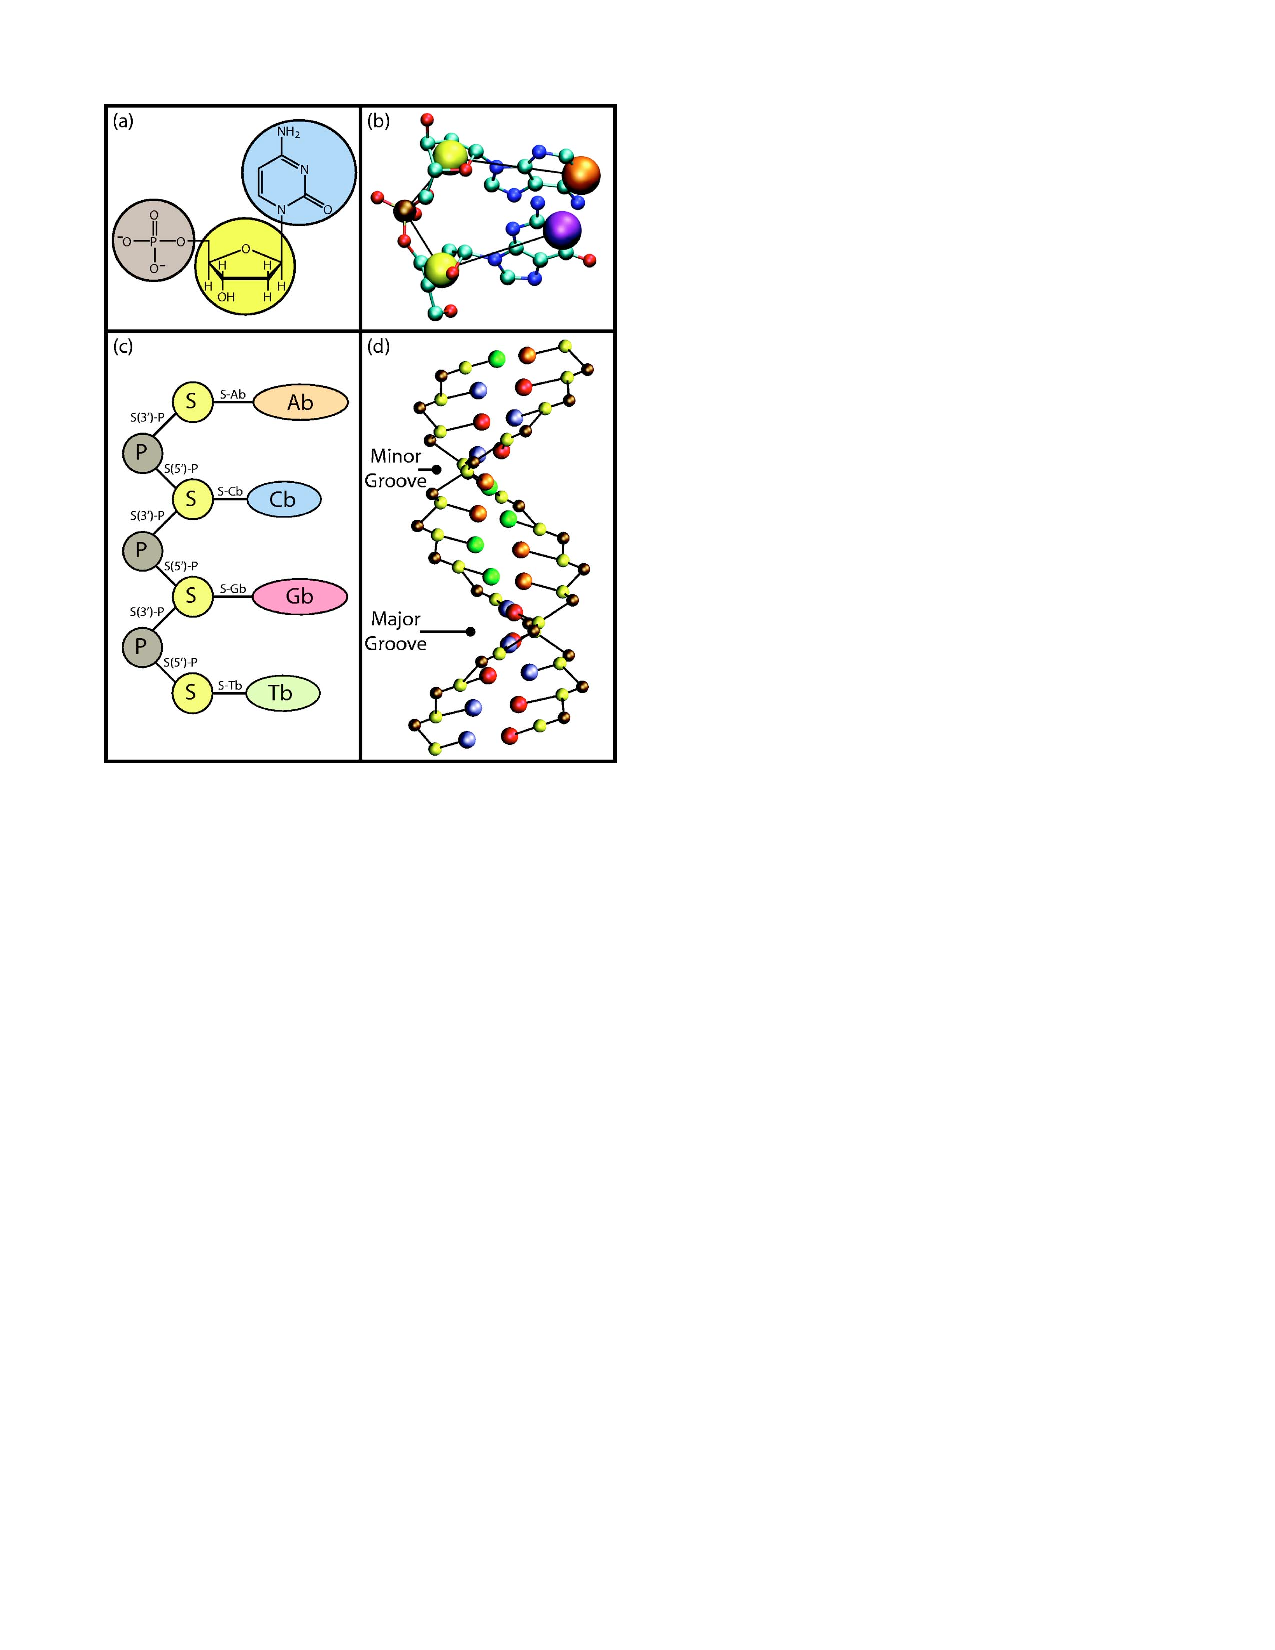
\includegraphics{images/schematic_structure_knotts}
\caption{The schematic structure of the model for B-DNA, from Knotts \etal \cite{knotts2007coarse}. Note the placing of the three sites per nucleus relative to the original atomic structure in the upper right panel.}
\label{schematic_knotts}
\end{center}
\end{figure}

\begin{figure}[h]
\begin{center}
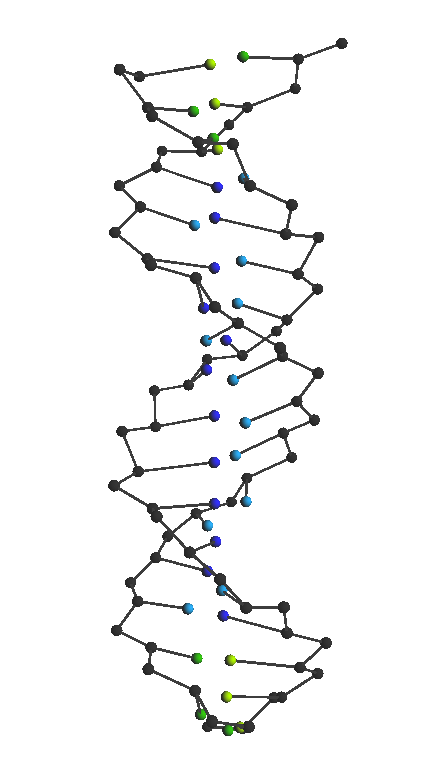
\includegraphics[width=5cm]{images/methods_dnaStructure1} 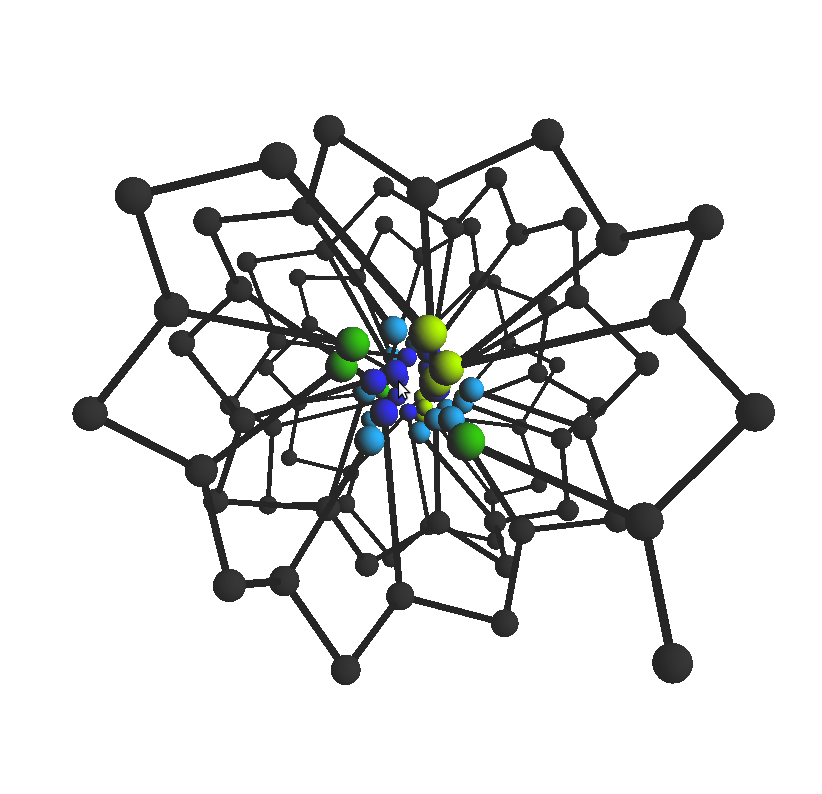
\includegraphics[width=7cm]{images/methods_dnaStructure2}

\end{center}\label{methods_dnaStructure}
\caption{Side- and top view of the dsDNA structure in our implemented model. The major and minor groove structure in the double helix is clearly visible; as is the screw symmetry from the top view.}
\end{figure}





\subsection{Interactions}

Interactions between the sites are modelled through several potential energies.
These potentials are taken taken mainly from the potential terms as defined by Florescu \& Joyeux \cite{florescu2011thermal}, and are an improvement over the original terms by Knotts \etal \cite{knotts2007coarse}. Deviations from \cite{florescu2011thermal} will be explicitly mentioned. The world simulated has periodic boundary conditions, with a world size (width, height, depth) taken to be a monomer length factor (default $5$ \Angstrom) times the number of monomers in a single strand.

We will now sketch the specific potential energy terms, one by one.

\begin{table}[hbt]
\begin{center}
\caption{Coupling constants for the various potentials. The basic energy unit $\varepsilon$ is equal to $0.26$\,kcal/mol, or $1.81 \times 10^{-21}$\,J.
We adopted the updated base pairing strenghts of Florescu \& Joyeux \cite{florescu2011thermal}.}
\begin{tabular}{cc||cc}
Parameter & Value & Parameter & Value\\\hline
$k_1$ & $\varepsilon$ per $\Angstrom^2$ &
	$k_\phi$ & $4\varepsilon$ \\
$k_2$ & $100\varepsilon$ per $\Angstrom^2$ &
	$\epsAT$ & 3.90\,kcal/mol\\
$k_\theta$ & $400\varepsilon$ per (radian)$^2$ &
	$\epsGC$ & 4.37\,kcal/mol\\
\end{tabular}\label{couplingConstants}
\end{center}
\end{table}


\paragraph{Bond potential}
The intramolecular bonds between connected sites in the same DNA strand is modelled by the potential
\begin{equation}
\Vbond
= \sum_{\substack{\text{bound sites}\\i}} \left[
	k_1 \left(d_i - d_{0_i}\right)^2
	+ k_2 \left(d_i - d_{0_i}\right)^4
\right],
\end{equation}
where $d_i$ is the distance between the sites that constitute the $i$th bond and $d_{0_i}$ is the equilibrium distances for that bonds, as determined by the standard B-form structure of double strand DNA. The explicit values of these equilibrium distances and of the coupling constants $k_1$ and $k_2$ can be found it table \ref{geometricConstants} and \ref{couplingConstants}, respectively.


\paragraph{Bond angle potential}
The angle $\theta$ that forms between three consecutively bound sites in a DNA strand is regulated by the harmonic potential
\begin{equation}
\Vang
= \sum_{\substack{\text{angle triplets}\\i}}
	\frac{k_\theta}{2} \left(
		\theta_i - \theta_{0_i}
	\right)^2,
\end{equation}
where the equilibrium angle $\theta_{0_i}$ is defined from the DNA B-form (values are tabulated in table \ref{geometricConstants}). The coupling constant $k_\theta$ is defined in table \ref{couplingConstants}.


\paragraph{Dihedral angle potential}
This potential regulates the dihedral angle $\phi$ between four consecutive bound sites on the same strand. It is given by
\begin{equation}
\Vdih
= \sum_{\substack{\text{dihedrals}\\i}}
	k_\phi \left[ 1 - \cos (\phi_i - \phi_{0_i}) \right],
\end{equation}
with $\phi_{0_i}$ the equilibrium dihedral angle from the DNA B-form definitions. The constants are defined in tables \ref{geometricConstants} and \ref{couplingConstants}.


\paragraph{Stacking potential}
The stacking potential is a Lennard-Jones type potential describing the intra-strand base stacking phenomena. It helps regulate the rigidity of the DNA backbone:
\begin{equation}
\Vstck
= \sum_{\substack{\text{stack pairs}\\i}}
	\varepsilon \left[
       		   \left(\frac{\dstck_i}{r_i} \right)^{12}
       		- 2\left(\frac{\dstck_i}{r_i} \right)^{6}
       	\right],
\end{equation}
where $r_i$ is the distance between the bases of the stacking pair. The sum over stack pairs runs between the $i$th and $(i+1)$th base, but also between the $i$th and $(i+2)$th base of the same strand.
This corresponds to an (off latice) G$\bar{\text o}$-type native contact scheme\cite{hoangcieplak, cieplak2003folding} with a cut-off distance of $9$\,\Angstrom.

The equilibrium distances $d_{ij}^\text{stck}$ are determined from the B isoform data in table \ref{dnaStructureData}.


\paragraph{Base pairing potential}
A hydrogen bonding interaction between two complimentary bases is modelled by
\begin{equation}
\Vbp
= \sum_{\substack{\text{base pairs}\\i}}
\varepsilon^\text{bp}_i \left[
	  5\left(\frac{\dbp_i}{r_i} \right)^{12}
	- 6\left(\frac{\dbp_i}{r_i} \right)^{10}
\right]
\end{equation}
where the equilibrium distances $d^\text{bp}_i$ and coupling constants $\varepsilon^\text{bp}_i$ depend on the type base pair. The explicit values are given in table \ref{couplingConstants}. No interaction is assumed between non-complementary base pairs.

Following Florescu \& Joyeux \cite{florescu2011thermal}, we only allow base pairing between the corresponding base on the other strand when simulating dsDNA. Likewise, when simulating hairpins, only interactions between the matching `mirrorred' bases are allowed. This facilitates renaturation and hairpin zipping when we want to simulate the scaling laws thereof. It also avoids the unphysical situation where a single base forms hydrogen bonds with multiple other bases. However, because there are now less potential bindings, the interaction strenghts will need to be increased in order to retain the correct critical temperatures. We used the ajusted strenghts determined in \cite{florescu2011thermal}.


\paragraph{Coulombic potential}
The final potential in our model is the screened electrostatic Coulomb interaction between the charged phosphate groups situated on the backbone of the DNA strands. It is modeled using a Debye-H\"uckel approximation with a Debye length $\kappa_D$ depending on the salt concentration of the environment,
\begin{equation}
\Vqq
= \sum_{\substack{\text{phosphate pairs}\\i}}
	\frac{e^2}{4 \pi \varepsilon_0 \varepsilon_k r_i}
       		\exp \left(- \frac{r_i}{k_D} \right),
\label{Vcoulomb}
\end{equation}
where the Debye length can be written as
\begin{equation}
\kappa_D
= \sqrt{ \frac{\varepsilon_0 \varepsilon_k RT}{2N^2_A e^2 I}}
\end{equation}
where we use the vacuum permittivity $\varepsilon_0$, Avogadro's number $N_A$, the elementary electric charge $e$ and the ionic strength $I$. For a realistic value of the ionic strength $[\text{Na}^+] = 50$\,mM (milimolair, equal to milimol/liter) this yields $\kappa_D$ = 13.603\,\Angstrom. The remaining constant in \eqref{Vcoulomb} is the dielectric constant $\varepsilon_k = 80$ for water at room temperature.


\paragraph{Exclusion potential}
Steric repulsion between sites is modelled using the repulsive part of a Lennard-Jones potential
\begin{equation}
\Vexcl
= \sum_{\substack{\text{exclusion pairs}\\i}}
\begin{cases}
	\varepsilon \left[
		   \left(\dfrac{\dexcl_i}{r_i} \right)^{12}
		- 2\left(\dfrac{\dexcl_i}{r_i} \right)^{6}
       	\right] + \varepsilon
	\qquad &\text{if }r_i < \dexcl_i,\\
	0
	\qquad &\text{if }r_i \geq \dexcl_i.
\end{cases}
\end{equation}
A pair of sites (not necessarily on the same strand) is considered an `exclusion pair' if it does not form a bond (in the sense of contributing to \Vbond).
The cut off distances $\dexcl_i$ are set to $1\,\Angstrom$ for exclusion between base pairs, and $5.5\,\Angstrom$ between all other base pairs.

In the original and follow-up versions of the 3SPN model (Knotts \etal \cite{knotts2007coarse}, Sambriski \etal \cite{sambriski2009mesoscale}), the cut off distance between non-base pairs was set to the higher value of $6.86\,\Angstrom$. However, this value causes some artificial swelling of the DNA strand beyond its equilibrium B form. We therefore opted to lower this exclusion cut off, effectively reducing the steric radius of the sites. For a value of $5.5\,\Angstrom$, the equilibrium distances between the sites are fully determined by the equilibrium constants in \Vbond and there is no swelling.

Note that Florescu \& Joyeux \cite{florescu2011thermal} reported that the exclusion potential does not play a significant role when simulating melting temperatures and renaturation properties of long double stranded DNA helices. They opted to leave it out altogether.

However, we are interested in the scaling behaviour of DNA hairpin zipping time and, as mentioned in the introduction, the helical nature of DNA might play a crucial role in that case \cite{carlon2010unwinding}.
In this spirit, we held on to the exclusion interaction. Note that we verified that our reduced steric cut off distance of $5.5\,\Angstrom$ is still sufficient to forbid overlap between (and passage through) DNA strands. Hence, the strands will indeed be forced to rotate during (de)naturation.


\paragraph{Total potential}
The total interaction is not merely a sum of the individual terms.
Following Knotts \etal\ \cite{knotts2007coarse}, two sites are excluded from non-bonded interactions (\Vstck, \Vbp, \Vqq, \Vexcl) if they constitute a bond (as per \Vbond).

On top of that, \Vbp, \Vqq\ and \Vexcl\ are modeled as mutually exclusive, where the exclusion force has the lowest precedence (note that base pairing and Coulomb repulsion cannot happen simultaneously between the same two sites).
Indeed, the exclusion force merely acts to keep two sites from passing through each other, something that is already achieved by the base pairing and Coulomb repulsion.

Because non-bonded potentials are short ranged, we can truncate them at a sufficiently large distance.
This enables us to work with a space partitioning acceleration scheme discussed below.
We chose to truncate the potentials at a distance of $20\,\Angstrom$. After truncation, the potentials are shifted so they yield a potential energy of zero when calculated at (and beyond) the truncation distance.



\begin{table}[htb]
\caption{Geometric constants for the potential energy functions as defined above. Important to note is that a phosphate can bind to a sugar at the 5' or the 3' carbon. The table is reproduced from Knotts \etal \cite{knotts2007coarse}, with our own value for \dexcl\ and following Florescu \& Joyeux for the base pairing strengths \cite{florescu2011thermal}.}
\begin{center}
\begin{tabular}{cc@{\qquad}cc}
Bond& $d_0$ (\Angstrom) & Bond Angle&     $\theta_0$ (degree) \\\hline
S(5')--P & 3.899 &        S(5')--P--(3')S & 94.49\\
S(3')--P & 3.559 &        P--(5')S(3')--P & 120.15 \\
S--Ab    & 6.430 &        P--(5')S--Ab    & 113.13\\
S--Tb    & 4.880 &        P--(3')S--Ab    & 108.38\\
S--Cb    & 4.921 &        P--(5')S--Tb    & 102.79\\
S--Gb    & 6.392 &        P--(3')S--Tb    & 112.72\\
&&                        P--(5')S--Cb    & 103.49\\
&&                        P--(3')S--Cb    & 112.39\\
&&                        P--(5')S--Gb    & 113.52\\
&&                        P--(3')S--Gb    & 108.12\\
& & & \\
Dihedral Angle & $\phi_0$ (degree) & Nonbonded & Length (\Angstrom) \\
\hline
P-(5')S(3')-P-(5')S & $-154.80$&   $\dstck$ & Derived from table \ref{geometricConstants} \\
S(3')-P-(5')S(3')-P & $-179.17$&   & \\  
Ab-S(3')-P-(5')S &    $ -22.60$&   $\dbp_\text{AT}$ & $2.9002$ \\
S(3')-P-(5')S-Ab &    $  50.69$&   $\dbp_\text{GC}$ & $2.8694$ \\ 
Tb-S(3')-P-(5')S &    $ -33.42$&   & \\
S(3')-P-(5')S-Tb &    $  54.69$&   $\dexcl$         & $1.0$ (mismatched bases) \\
Cb-S(3')-P-(5')S &    $ -32.72$&   $\dexcl$         & $5.5$ (otherwise) \\
S(3')-P-(5')S-Cb &    $  54.50$&   & \\
Gb-S(3')-P-(5')S &    $ -22.30$&   & \\
S(3')-P-(5')S-Gb &    $  50.66$&   & 
\end{tabular}\label{geometricConstants}
\end{center}
\end{table}



\subsection{Space Partitioning}

\subsubsection{General idea}
A naive implementation of non-bonded forces would test every possible pair of particles, for a total of $n(n-1)/2$ possibilities, with $n$ the number of interacting particles (for our coarse grained DNA model, $n$ would be the number of sites, which is three times the number of monomers).
However, most of these considered pairs are superfluous because the particles are separated too far apart and their interaction is negligible. This $O\left(\frac{n(n-1)}{2}\right) = O(n^2)$ complexity is undesirable for performance reasons.
A known technique to improve this algorithmic complexity is called \emph{spatial partitioning}. An explanation (and application to multiprocessor scaling) can, for instance, be found in \cite{plimpton1995fast}.

By splitting the world into smaller partitions, or \emph{boxes}, one only has to check for interactions between particles in nearby partitions.
In the ideal case, if the number of interacting particles contained per box is a constant $x$, the amount of boxes becomes $n/x$. Interactions need only be checked between particles in the same box for $x(x-1)/2$ pairs, and between particles in a given box and particles in the adjacent boxes. If each box has $z$ neighbouring boxes, then there are $zx^2/2$ such pairs. The total complexity of this problem thus reduces to 
$O\left(
	\left[ \frac{x(x-1)}{2} + \frac{zx^2}{2} \right]
		\cdot \frac{n}{x}
\right) = O(n)$,
linear in the number of interacting particles.

It is easy to show that we cannot do any better than $O(n)$ via this partitioning trick, and that choosing the number of boxes $b$ to be proportional to $n$ is the ideal case.
Indeed, assume that we would instead take the number of boxes $b \sim n^\alpha$. Then the average number of particles per box $x$ would be proportional to $n^{1 - \alpha}$. Using the reasoning above, we find that the average number of interaction pairs that would be considered is proportional to $x^2 b = n^{2(1 - \alpha)} n^\alpha = n^{2 -\alpha}$. It seems that we can make the algorithmic complexity sub-linear by choosing $\alpha > 1$, however, we also have to iterate over all the boxes, and their number is proportional to $n^\alpha$. In other words, the total algorithmic time complexity is $O(n^{2 - \alpha} + n^\alpha)$, with the optimal value of $\alpha$ equal to one.


\subsubsection{Applied to DNA}



\subsection{Dynamics}
We implemented the velocity Verlet algorithm and a Langevin integrator. The velocity Verlet algorithm was used to check the correctness of the potentials and interaction forces by means of energy conservation when not coupled to an external heat bath. All actual simulations were carried out using the Langevin integrator.

The Langevin integrator is a variant of the BBK type integrator due to Br{\"u}nger, Brooks and Karplus \cite{brunger1984stochastic}. Using a velocity Verlet style algorithm, the Langevin equation
\begin{equation}
m a(t) = F(t) - \gamma m v(t) + R(t)
\end{equation}
is discretized and integrated. Here, $\gamma$ is a friction coefficient and $R(t)$ is a gaussian stochastic force with correlation function $\langle\gamma(t), \gamma(t')\rangle = 2 m k_\text{B} T \gamma \delta(t-t')$.

At each iteration, the velocities $v$ first get updated by a half timestep
\begin{equation}
v\left(t + \frac{\Delta t}{2}\right)
= \left(1 - \gamma\frac{\Delta t}{2}\right) v(t)
	+ \frac{\Delta t}{2m} [F(t) + R(t)],
\end{equation}
after which the positions $r$ can be updated to
\begin{equation}
r(t + \Delta t)
= r(t) + v\left(t + \frac{\Delta t}{2}\right) \Delta t.
\end{equation}
With the positions updated, the new forces $F$ can be calculated. With these forces, the velocities can once again be half stepped according to
\begin{equation}
v(t + \Delta t) = \left(1 + \gamma \frac{\Delta t}{2}\right)^{-1}
\left\{
	v\left(t + \frac{\Delta t}{2}\right)
	+ \frac{\Delta t}{2m} \left[
			F(t + \Delta t) + R(t + \Delta t)
	\right]
\right\}.
\end{equation}
The discretized random force $R$ is given by a gaussian random variable with variance $2 m k_\text{B} T \gamma / \Delta t$.

The appropriate friction coefficient was determined by comparing simulated diffusion constants with experimental data. We ended up on a value of $\gamma = 5 \times 10^{12} s^{-1}$, yielding a diffusion coefficient of $(1.3 \pm 0.1) \times 10^{-10}$\,m$^2$/s for a 12 base pair single strand of Adenine at 300\,K and a salt concentration of $[\text{Na}^+] = 50$\,mM.
Figure \ref{diffusion} shows the squared displacements of the simulations that were performed to achieve this result. This is in good agreement with the experimentally determined value of $(1.34 \pm 0.09) \times 10^{-10}$\,m$^2$/s \cite{stellwagen2001measuring, bonifacio1997comparison, eimer1991rotational}. 

\begin{figure}[htb]
       \begin{center}
               \scalebox{0.9}{
                        \nonstopmode
                        % GNUPLOT: LaTeX picture with Postscript
\begingroup
  \makeatletter
  \providecommand\color[2][]{%
    \GenericError{(gnuplot) \space\space\space\@spaces}{%
      Package color not loaded in conjunction with
      terminal option `colourtext'%
    }{See the gnuplot documentation for explanation.%
    }{Either use 'blacktext' in gnuplot or load the package
      color.sty in LaTeX.}%
    \renewcommand\color[2][]{}%
  }%
  \providecommand\includegraphics[2][]{%
    \GenericError{(gnuplot) \space\space\space\@spaces}{%
      Package graphicx or graphics not loaded%
    }{See the gnuplot documentation for explanation.%
    }{The gnuplot epslatex terminal needs graphicx.sty or graphics.sty.}%
    \renewcommand\includegraphics[2][]{}%
  }%
  \providecommand\rotatebox[2]{#2}%
  \@ifundefined{ifGPcolor}{%
    \newif\ifGPcolor
    \GPcolortrue
  }{}%
  \@ifundefined{ifGPblacktext}{%
    \newif\ifGPblacktext
    \GPblacktexttrue
  }{}%
  % define a \g@addto@macro without @ in the name:
  \let\gplgaddtomacro\g@addto@macro
  % define empty templates for all commands taking text:
  \gdef\gplbacktext{}%
  \gdef\gplfronttext{}%
  \makeatother
  \ifGPblacktext
    % no textcolor at all
    \def\colorrgb#1{}%
    \def\colorgray#1{}%
  \else
    % gray or color?
    \ifGPcolor
      \def\colorrgb#1{\color[rgb]{#1}}%
      \def\colorgray#1{\color[gray]{#1}}%
      \expandafter\def\csname LTw\endcsname{\color{white}}%
      \expandafter\def\csname LTb\endcsname{\color{black}}%
      \expandafter\def\csname LTa\endcsname{\color{black}}%
      \expandafter\def\csname LT0\endcsname{\color[rgb]{1,0,0}}%
      \expandafter\def\csname LT1\endcsname{\color[rgb]{0,1,0}}%
      \expandafter\def\csname LT2\endcsname{\color[rgb]{0,0,1}}%
      \expandafter\def\csname LT3\endcsname{\color[rgb]{1,0,1}}%
      \expandafter\def\csname LT4\endcsname{\color[rgb]{0,1,1}}%
      \expandafter\def\csname LT5\endcsname{\color[rgb]{1,1,0}}%
      \expandafter\def\csname LT6\endcsname{\color[rgb]{0,0,0}}%
      \expandafter\def\csname LT7\endcsname{\color[rgb]{1,0.3,0}}%
      \expandafter\def\csname LT8\endcsname{\color[rgb]{0.5,0.5,0.5}}%
    \else
      % gray
      \def\colorrgb#1{\color{black}}%
      \def\colorgray#1{\color[gray]{#1}}%
      \expandafter\def\csname LTw\endcsname{\color{white}}%
      \expandafter\def\csname LTb\endcsname{\color{black}}%
      \expandafter\def\csname LTa\endcsname{\color{black}}%
      \expandafter\def\csname LT0\endcsname{\color{black}}%
      \expandafter\def\csname LT1\endcsname{\color{black}}%
      \expandafter\def\csname LT2\endcsname{\color{black}}%
      \expandafter\def\csname LT3\endcsname{\color{black}}%
      \expandafter\def\csname LT4\endcsname{\color{black}}%
      \expandafter\def\csname LT5\endcsname{\color{black}}%
      \expandafter\def\csname LT6\endcsname{\color{black}}%
      \expandafter\def\csname LT7\endcsname{\color{black}}%
      \expandafter\def\csname LT8\endcsname{\color{black}}%
    \fi
  \fi
  \setlength{\unitlength}{0.0500bp}%
  \begin{picture}(9600.00,7680.00)%
    \gplgaddtomacro\gplbacktext{%
      \colorrgb{0.00,0.00,0.00}%
      \put(1116,845){\makebox(0,0)[r]{\strut{}0}}%
      \colorrgb{0.00,0.00,0.00}%
      \put(1116,2097){\makebox(0,0)[r]{\strut{}0.5}}%
      \colorrgb{0.00,0.00,0.00}%
      \put(1116,3348){\makebox(0,0)[r]{\strut{}1}}%
      \colorrgb{0.00,0.00,0.00}%
      \put(1116,4600){\makebox(0,0)[r]{\strut{}1.5}}%
      \colorrgb{0.00,0.00,0.00}%
      \put(1116,5851){\makebox(0,0)[r]{\strut{}2}}%
      \colorrgb{0.00,0.00,0.00}%
      \put(1116,7103){\makebox(0,0)[r]{\strut{}2.5}}%
      \colorrgb{0.00,0.00,0.00}%
      \put(1248,625){\makebox(0,0){\strut{}0}}%
      \colorrgb{0.00,0.00,0.00}%
      \put(2736,625){\makebox(0,0){\strut{}0.2}}%
      \colorrgb{0.00,0.00,0.00}%
      \put(4224,625){\makebox(0,0){\strut{}0.4}}%
      \colorrgb{0.00,0.00,0.00}%
      \put(5712,625){\makebox(0,0){\strut{}0.6}}%
      \colorrgb{0.00,0.00,0.00}%
      \put(7200,625){\makebox(0,0){\strut{}0.8}}%
      \colorrgb{0.00,0.00,0.00}%
      \put(8688,625){\makebox(0,0){\strut{}1}}%
      \colorrgb{0.00,0.00,0.00}%
      \put(478,3974){\rotatebox{90}{\makebox(0,0){\strut{}\rule{0pt}{-1.5cm}squared displacement ($10^{15}$\,m$^2$)}}}%
      \colorrgb{0.00,0.00,0.00}%
      \put(4968,295){\makebox(0,0){\strut{}time ($\mu$s)}}%
    }%
    \gplgaddtomacro\gplfronttext{%
    }%
    \gplbacktext
    \put(0,0){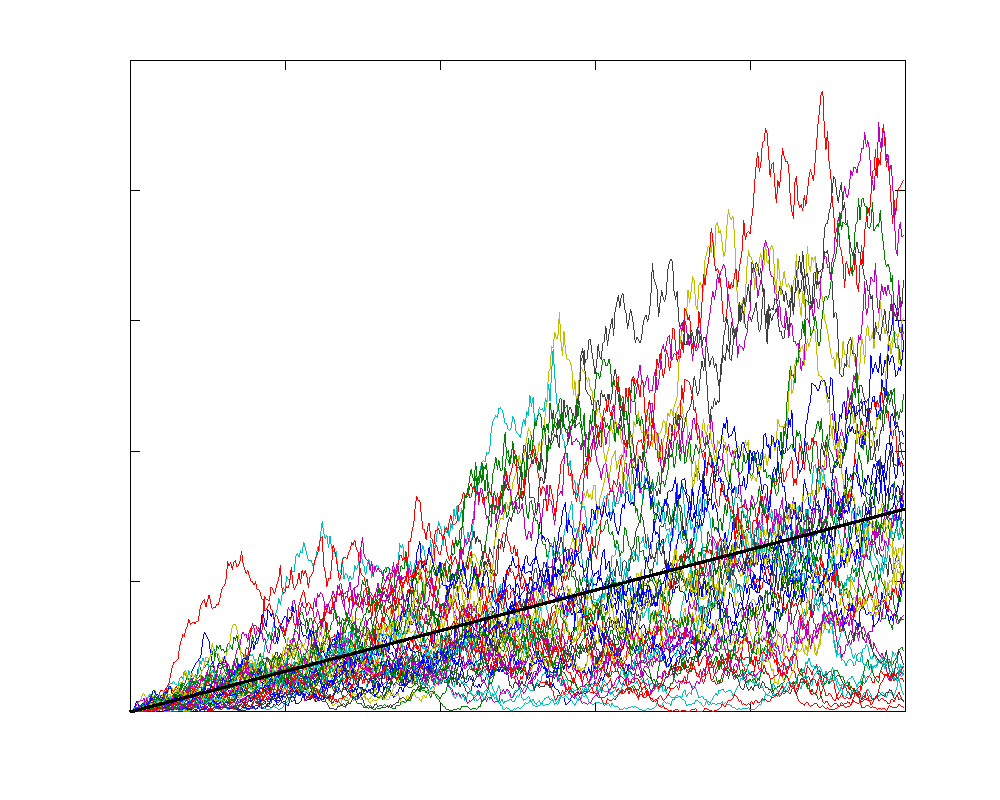
\includegraphics{images/diffusion}}%
    \gplfronttext
  \end{picture}%
\endgroup

                        \errorstopmode
                        \rule[-0.5cm]{0cm}{0cm}}
                \caption{Diffusion of a 12 monomer single strand of Adenine. Shown are the squared displacements of 45 individual simulations at 300\,K and with friction $\gamma = 5 \times 10^{12}$. The black line is the $6Dt$ mean squared displacement curve for the fitted value of $D = (1.3 \pm 0.1) \times 10^{-10}$\,m$^2$/s.}
		\label{diffusion}
        \end{center}
\end{figure}






